\chapter{Výroba vodíku v rafinériích}

Vodík může být produkován z fosilních paliv, biomasy nebo vody, případně z jejich směsí. V současné době je hlavním zdrojem pro výrobu vodíku zemní plyn, který se využívá v parních reformátorech. Zemní plyn představuje zdroj přibližně $63\%$ celosvětové produkce vodíku (viz Obr. \ref{fig:produkceH2}), při které se spotřebuje až $205\krat10^{9}\ \mathrm{m^3}$ zemního plynu. Dalším významným zdrojem pro výrobu vodíku je uhlí, které má dominantní postavení zejména v Číně. \cite{Seddon2022}
Dle odhadů \acs{IEA} je známo, že uhlí přispívá k celosvětové produkci vodíku až $21\%$, přičemž se spotřebuje $205\ \mathrm{Mt}$ uhlí. V neposlední řadě lze vodík vyrábět také z ropných produktů, nebo meziproduktů které je výhodné zpracovávat rovnou v rafinériích. \cite{IEAfuture}

Přibližně dvě třetiny vyprodukovaného vodíku se vyrábějí přímo v rafineriích dále popsanými dostupnými technologiemi, nebo jsou získávány přímo od dodavatelů. \cite{IEAfuture} Zbývající třetinovou část pak tvoří získávání vodíku jako vedlejšího produktu při jiných technologiích probíhajících v rafinériích, především pak katalytickým reformingem. \cite{Blazek2006}

\section{Parní reformování zemního plynu}

Využívání technologie parního reformování metanu (\acs{SMR}), nebo vyšších uhlovodíků, se rozšířilo s dostupností zemního plynu ve vyspělých zemích kolem 60. let minulého století, kdy nahradila technologie založené na zpracovávání uhlí. Hlavní výhodou parního reformování je vlastnost metanu v přítomnosti kyslíku, nebo častěji používané vody tvořit při vysokých teplotách směs oxidu uhličitého a vodíku, nebo oxidu uhelnatého a vodíku. \cite{Seddon2022} 
\reaction{CH4 + H2O <-> CO + 3H2}
\reaction{CH4 + 2H2O <-> CO2 + 4H2}
Tyto reakce jsou vysoce endotermní a probíhají v přítomnosti katalyzátoru na bázi niklu při následujících reakčních parametrech
\begin{table}[h]
    \centering
    \begin{tabular}{|c|c|}
        \hline
        \textbf{Parametr reakce} & \textbf{Hodnoty a jednotky} \\ \hline\hline
        Teplota & $750\div800\ \mathrm{^{\circ}C}$ \\ \hline
        Tlak & $3 \div 5\ \mathrm{MPa}$ \\ \hline
    \end{tabular}
    \caption[Reakční podmínky SMR]{Reakční podmínky SMR \cite{Blazek2006}.}
    \label{tab:rp_smr}
\end{table}

\noindent
Vzniklý oxid uhelnatý je ve dvojici vysokoteplotního a nízkoteplotního konvertoru v reakci s vodní párou přeměňován na oxid uhličitý a vodík. Tento proces je popsán následující exotermní reakcí \cite{Blazek2006}
\reaction{CO + H2O <-> CO2 + H2}
Oxid uhličitý je ve velké míře vypírán v absorbéru ze směsi. Vhledem k vysokým požadavkům na čistotu výstupního vodíku je nutné zbylý oxid uhličitý zpět převádět na metan v metanizéru. Tento poslední krok celého procesu výroby vodíku parním reformingem je založen na následující exotermní reakci, probíhající při teplotě $400\ \mathrm{^{\circ}C}$ \cite{Blazek2006}
\reaction{CO2 + 4H2 <-> CH4 + 2H2O}
Výše popsaný proces je graficky znázorněn na schématu jednotky parního reformingu na Obr. \ref{fig:smr_schema}. Jedná se o jednoduché stanice na výrobu vodíku, které se využívají v rafinériích např. ve Spojených státech amerických. \cite{Seddon2022,Byrum2021} Mají vysokou účinnost kvůli recyklaci vody, metanu a přebytečného tepla z některých reakcí. Parní reforming je jedním z nejrozšířenějších a nejvyvinutějších rafinérských procesů, který produkuje vodík o čistotě až $98\%$. \cite{Seddon2022,Blazek2006}
\begin{figure}[h]
    \centering
    \begin{tikzpicture}
\node[inner sep=0pt] (obrazek) at (0,0)
    {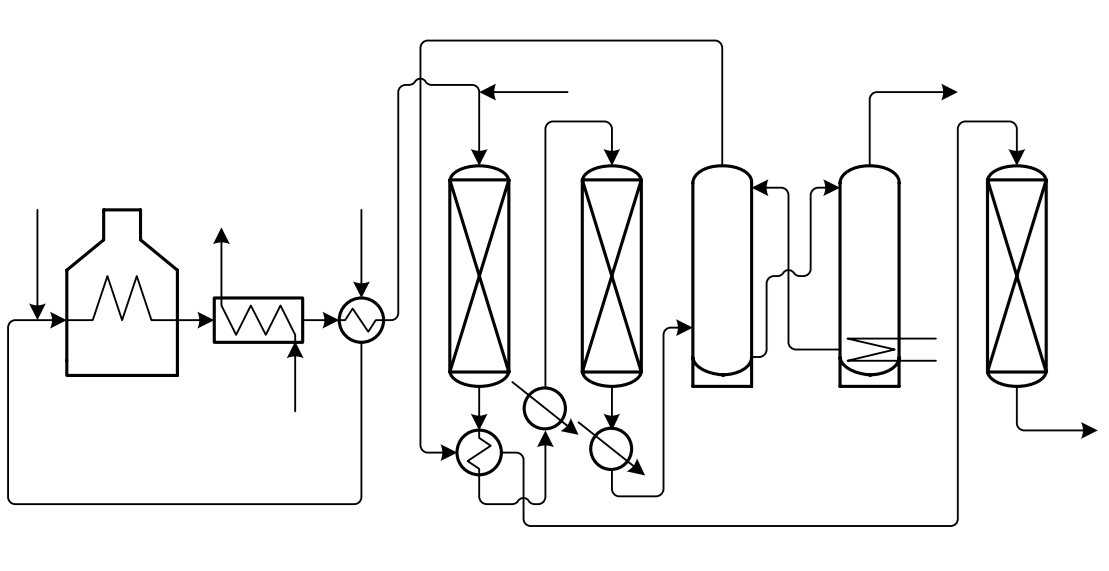
\includegraphics[width=0.8\textwidth]{figures/smr_schema.png}};
\node[font=\small\bfseries] at (-4.375,-0.6) {1};
\node[font=\small\bfseries] at (-3,0.2) {2};
\node[font=\small\bfseries] at (-0.75,0.85) {3};
\node[font=\small\bfseries] at (0.56,0.85) {4};
\node[font=\small\bfseries] at (1.7,0.85) {5};
\node[font=\small\bfseries] at (3.17,0.85) {6};
\node[font=\small\bfseries] at (4.67,0.85) {7};

\node[font=\scriptsize] at (-5.25,1) {pára};
\node[font=\scriptsize] at (-3.4,0.8) {pára};
\node[font=\scriptsize] at (0.55,1.95) {pára};
\node[font=\scriptsize,align=center] at (-2.08,1.24) {zemní\\plyn};
\node[font=\scriptsize] at (-2.6,-1.52) {voda};
\node[font=\scriptsize] at (3.5,2.2) {\ce{CO2}};
\node[font=\scriptsize] at (5,-1.75) {vodík};
\end{tikzpicture}
    \caption[Schéma parního reformování zemního plynu]{Schéma parního reformování zemního plynu \cite{Blazek2006}.\\(1 - pec, 2 - kotel na výrobu páry, 3 - vysokoteplotní konvertor \ce{CO}, 4 - nízkoteplotní konvertor \ce{CO}, 5 - absorbér \ce{CO2}, 6 - desorbér \ce{CO2}, 7 - metanizér)} \label{fig:smr_schema}
\end{figure}

\section{Parciální oxidace těžkých ropných frakcí}

Parciální, neboli částečnou, oxidací (\acs{POX}) rozumíme nekatalytické spalování uhlovodíků $\mathrm{C_nH_m}$ (těžkých ropných frakcí z předchozích rafinérských procesů) s kyslíkem. Za působení tepla a kyslíku dochází k destrukci uhlíkových vazeb až na metan. Zplyňování uhlovodíků je vysoce exotermní reakcí, která se dá realizovat následovně. \cite{Seddon2022,Blazek2006}
\reaction{2\mathrm{C_mH_n} + mO2 <-> 2mCO + nH2}
\reaction{\mathrm{C_mH_n} + mO2 <-> mCO2 + \frac{1}{2} nH2}
V případě zplyňování v přítomnosti vodní páry a kyslíku, část těžké ropné frakce reaguje s vodní párou za této endotermní reakce \cite{Blazek2006}
\reaction{\mathrm{C_mH_n} + mH2O <-> mCO + m + \frac{1}{2} nH2}
Tento způsob zplyňování vodní párou nejenže produkuje více vodíku ve srovnání s oxidačními reakcemi, ale zároveň snižuje teplotu vzniklých reakčních produktů z $1500\ \mathrm{^{\circ}C}$ na přibližně $1350\ \mathrm{^{\circ}C}$ při tlacích $3 \div 8\ \mathrm{MPa}$. Mezi nevýhody se naopak řadí produkce sazí a sazové vody.

Jednotky parciální oxidace se dimenzují na vysoký produkční výkon a jsou úspornější a levnější než jednotky parního reformingu. Důležitá je kvalita vstupního kyslíku, který musí být o čistotě $95 \div 99\%$. \cite{Seddon2022,Blazek2006} Schéma jednotky parciální oxidace na které se vodík vyrábí pomocí kyslíku a vodní páry je na Obr. \ref{fig:schema_pox}.
\begin{figure}[h]
    \centering
    \begin{tikzpicture}
\node[inner sep=0pt] (obrazek) at (0,0)
    {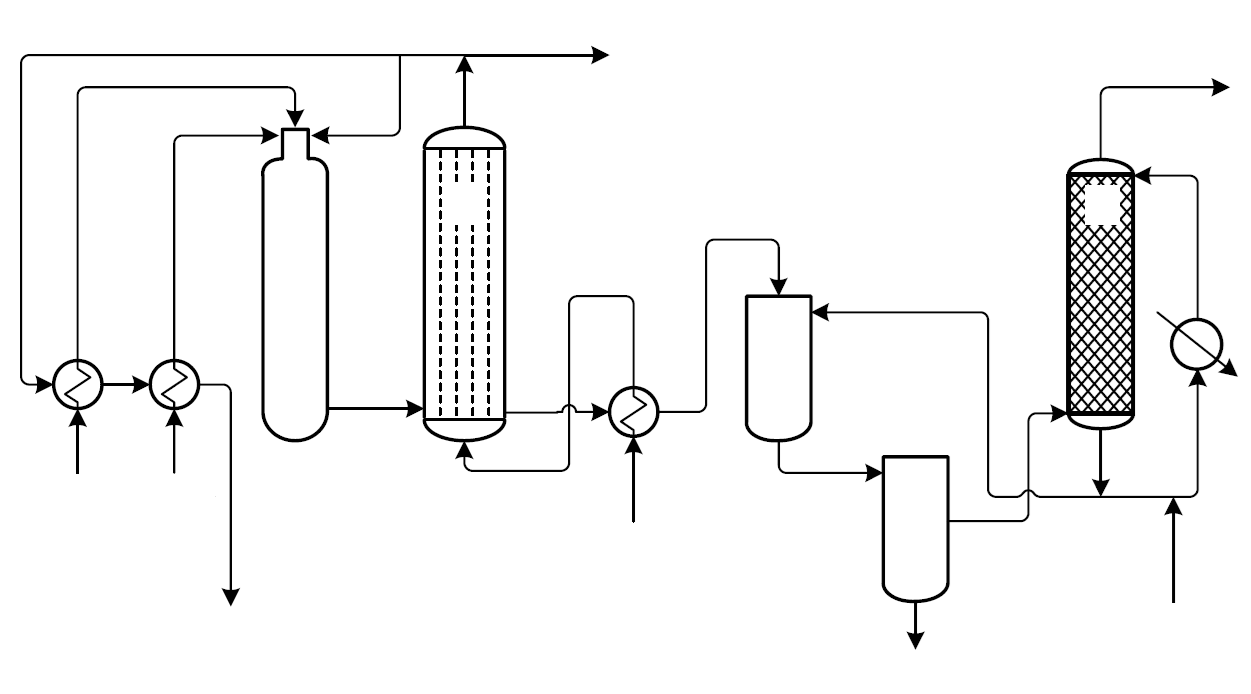
\includegraphics[width=0.8\textwidth]{figures/schema_pox.png}};
\node[font=\small\bfseries] at (-2.95,1.3) {1};
\node[font=\small\bfseries] at (-1.45,1.3) {2};
\node[font=\small\bfseries] at (1.36,0.1) {3};
\node[font=\small\bfseries] at (2.6,-1.4) {4};
\node[font=\small\bfseries] at (4.27,1.26) {5};

\node[font=\scriptsize,align=center] at (-4.9,-1.6) {těžký\\olej};
\node[font=\scriptsize] at (-4,-1.44) {kyslík};
\node[font=\scriptsize] at (-3.5,-2.55) {kondenzát};
\node[font=\scriptsize] at (-4,2.85) {vysokotlaká pára};
\node[font=\scriptsize] at (1.1,2.625) {vysokotlaká pára};
\node[font=\scriptsize,align=center] at (1.05,1.35) {surový\\plyn};
\node[font=\scriptsize,align=center] at (0.05,-1.95) {napájecí\\voda};
\node[font=\scriptsize] at (2.6,-2.9) {sazová voda};
\node[font=\scriptsize] at (4.9,-2.55) {voda};
\node[font=\scriptsize] at (5.1,1.75) {voda};
\node[font=\scriptsize] at (2.5,0.53) {voda};
\node[font=\scriptsize] at (4.4,2.6) {surový plyn};
\end{tikzpicture}
    \caption[Schéma parciální oxidace těžkých ropných olejů]{Schéma parciální oxidace těžkých ropných olejů \cite{Blazek2006}.\\(1 - zplyňovací reaktor, 2 - kotel na výrobu páry, 3 - chladič, 4 - separátor, 5 - pračka)} \label{fig:schema_pox}
\end{figure}

\noindent
Do cihlami vyzděného zplyňovacího reaktoru (\textbf{1}) se přivádí kyslík společně s párou a těžkou ropnou frakcí, odkud se po proběhnutí reakcí horké plyny předávají do kotle (\textbf{2}). V kotli se vytváří vysokotlaká pára, kolem které proudí proud plynů, který dále putuje přes chladič (\textbf{3}) a separátor sazí (\textbf{4}). Z vodní pračky (\textbf{5}) vychází surový syntézní plyn, který se dále zpracovává pro účely rafinérie (viz. kapitola \ref{sec:vyuziti_raf}). \cite{Seddon2022,Blazek2006}

\section{Elektrolýza vody}

Obě výše zmíněné možnosti výroby vodíku v rafinériích produkují vodík \textbf{šedý}. Jednotky parního reformování v rafinériích ve Spojených státech amerických, jsou k roku 2021 zodpovědné za $9\%$ všech vyprodukovaných emisí. Pro představu na $1\ \mathrm{kg}$ vyrobeného vodíku připadá zhruba $9 \div 12\ \mathrm{kg}$ vyprodukovaného oxidu uhličitého. \cite{Hytep} Možnou alternativou k částečnému omezení produkování emisí je přechod na výrobu \textbf{zeleného} vodíku elektrolýzou vody\footnote{Vodík lze požadovat za zelený pouze tehdy, když využívaní elektrická energie pochází z obnovitelných zdrojů - v případě rafinérií nejčastěji ze solárních panelů.}.

Elektrolýza vody je procesem výroby vodíku, při kterém se voda v roztoku s elektrolytem rozkládá na vodík a kyslík za působení elektrické energie ($\approx 240\ \mathrm{kJ\krat mol^{-1}}$) takto \cite{Kumar2022}
\reaction{2 H2O -> 2H2 + O2}
Během vývoje procesu elektrolýzy, který započal už v 19. století, byly objeveny a primárně aplikovány tři typy technologií vodní elektrolýzy. \cite{Kumar2022}
\begin{itemize}[leftmargin=*]
\item alkalická vodní elektrolýza
\item elektrolýza s protonově vodivou membránou (\acs{PEM})
\item elektrolýza s pevným oxidem\footnote{V češtině se častěji používá název \enquote{vysokoteplotní elektrolýza}.} (\acs{SOEC})
\end{itemize}
Princip dílčích technologií je stejný, avšak rozdíly jsou především v používání jiných elektrolytů, reakcí při jiných reakčních parametrů a vzniku iontů. \cite{Kumar2022}

Současná celková účinnost elektrolýzy vody se pohybuje mezi $50 \div 60\%$, v závislosti na použité technologii elektrolyzéru. K produkci $1\ \mathrm{kg}$ vodíku je zapotřebí přibližně $9\ \mathrm{l}$ demineralizované vody a zhruba $50\ \mathrm{kWh}$ elektrické energie. \cite{Hytep}

\subsection{Alkalická elektrolýza vody}

Alkalická elektrolýza vody je jeden z nejstarších a nejlépe zavedených technologií pro průmyslovou výrobu vodíku. Alkalická elektrolýza probíhá při relativně nízkých teplotách ($70\div90\ \mathrm{^{\circ}C}$) za přivádění elektrolytu ve formě koncentrovaného hydroxidu draselného (\ce{KOH}). Při napájení stejnosměrným proudem dochází na straně katody k redukci roztoku vody a elektrolytu na vodík. Na cestě k anodové straně prochází vzniklé hydroxidy (\ce{OH-}), které fungují jako nosič iontového náboje, porézní membránou z kompozitních materiálů, která zprostředkovává elektrochemickou reakci. Na straně anody dochází k oxidaci hydroxylových iontů na vodu a kyslík. \cite{Tkac2017,Kumar2022}
\begin{figure}[h]
    \centering
    \begin{tikzpicture}
\node[inner sep=0pt] (obrazek) at (0,0)
    {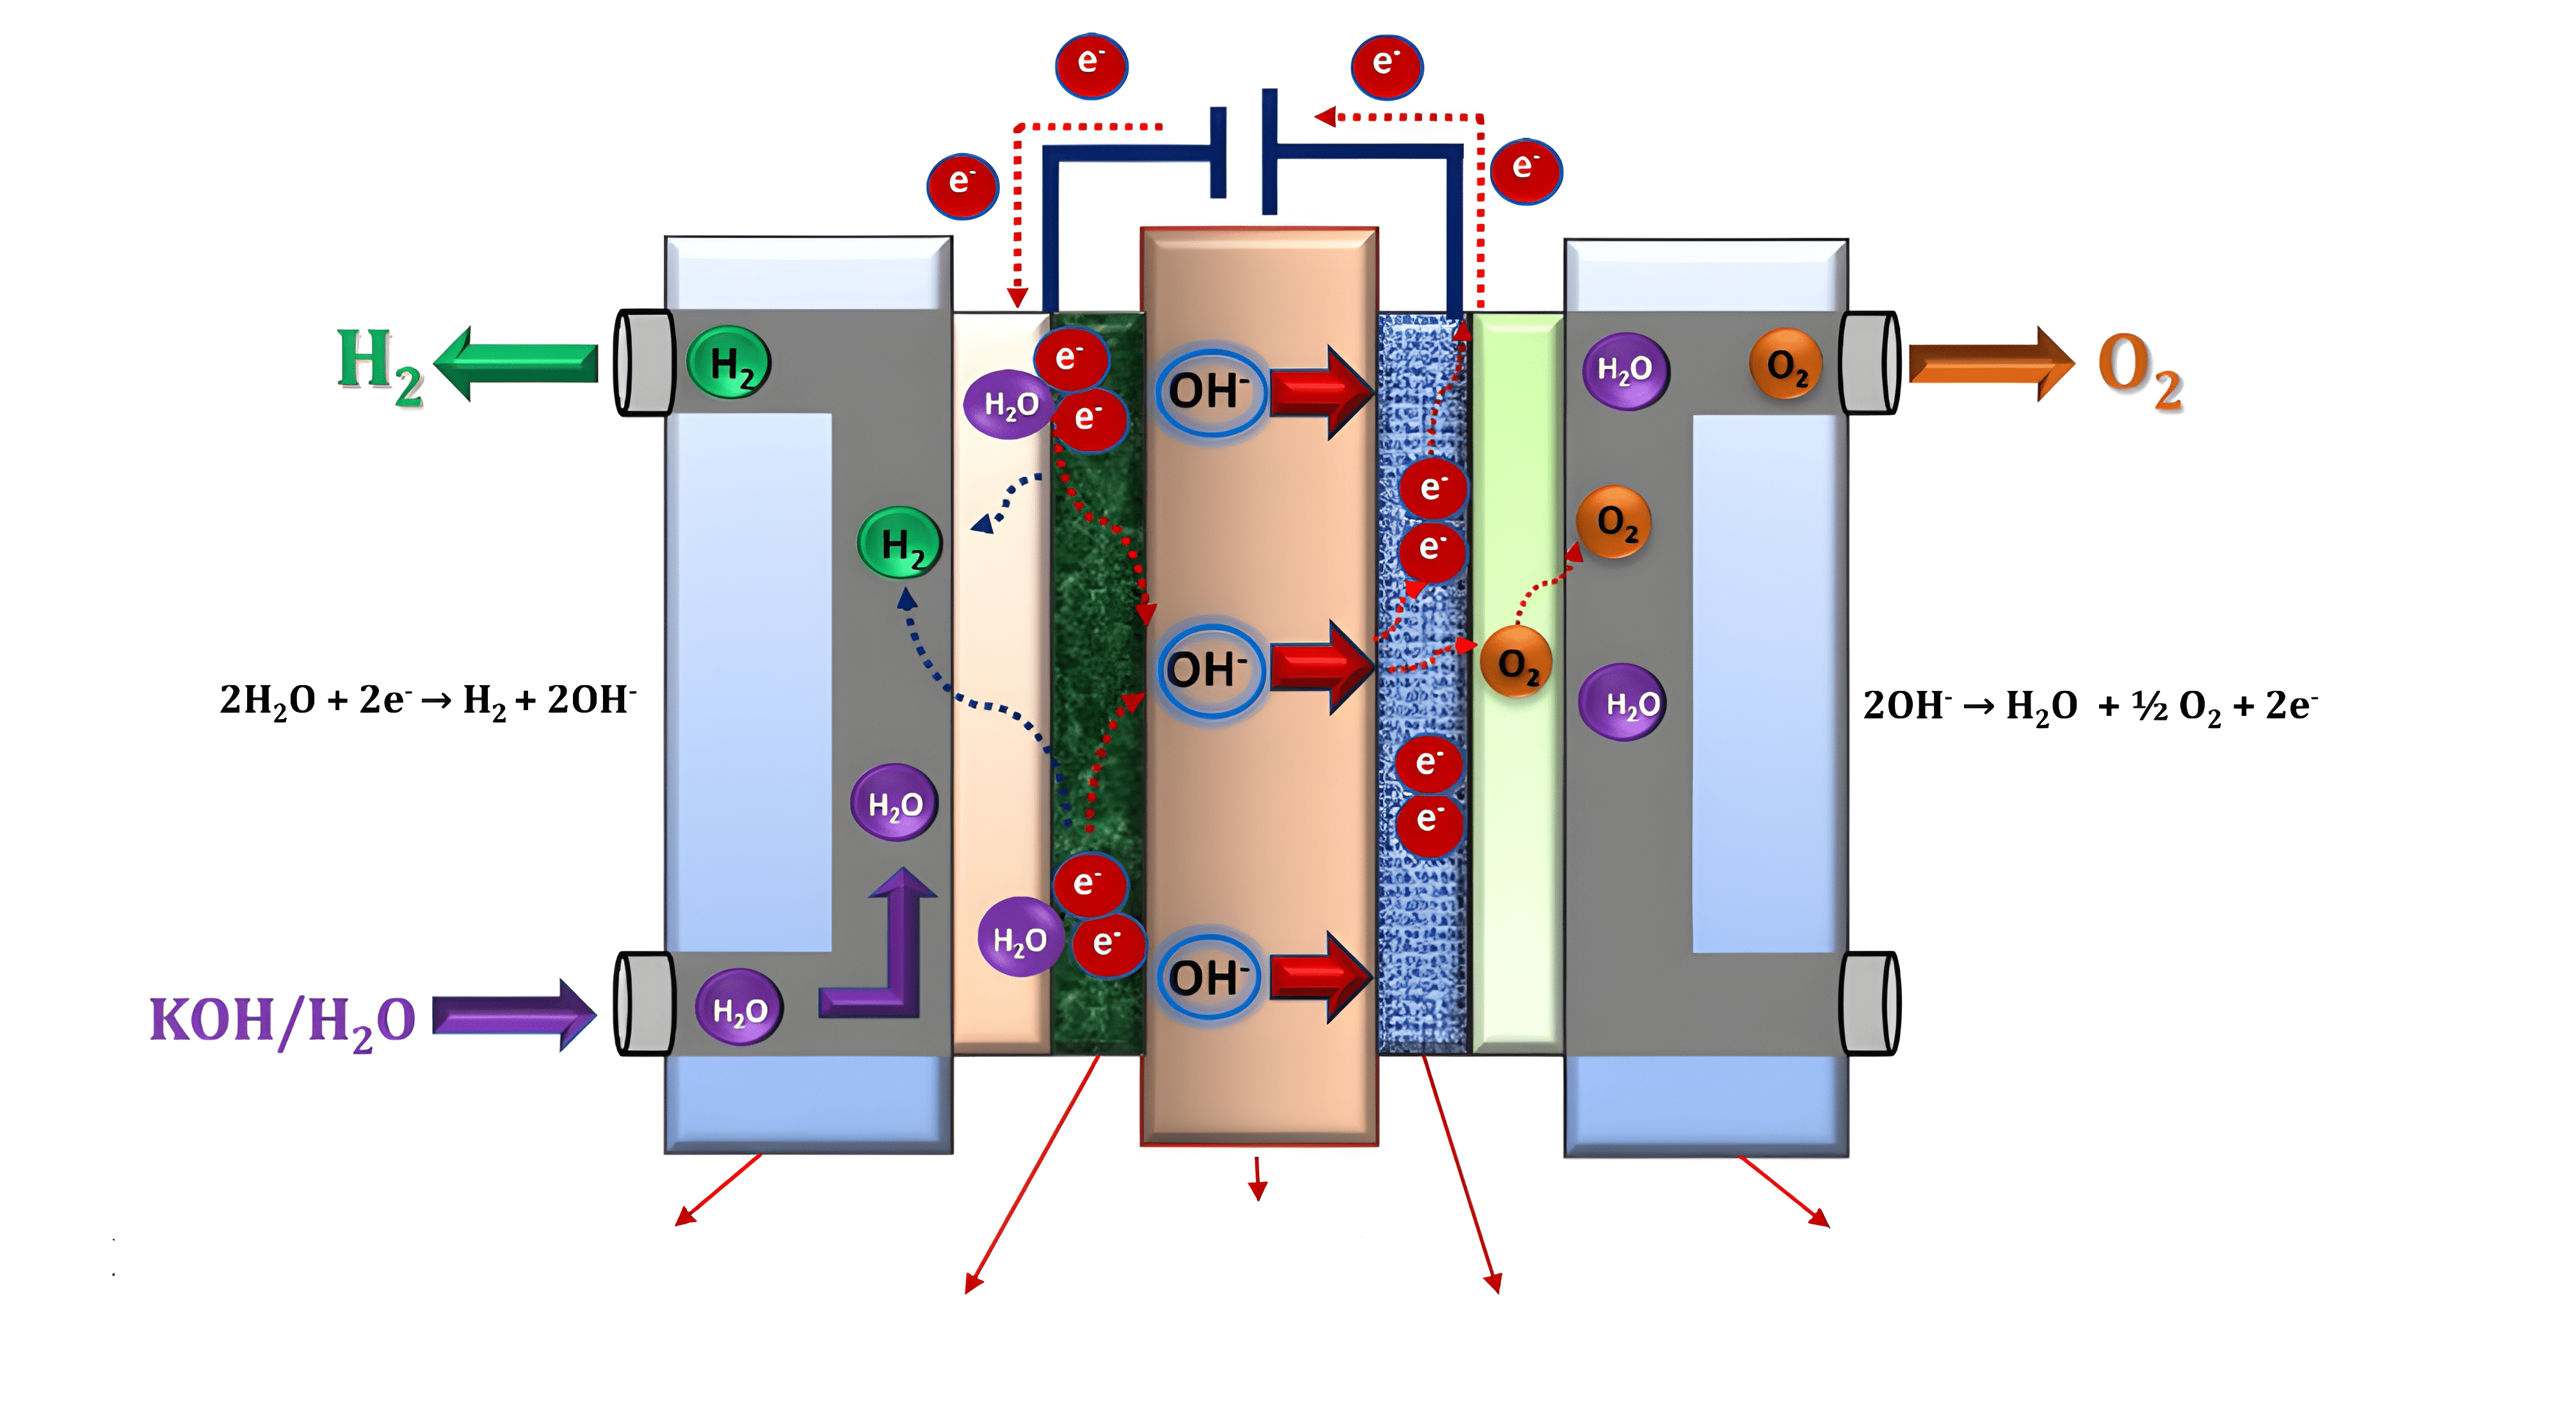
\includegraphics[width=0.9\textwidth]{figures/elekt_alk.png}};
\node[font=\scriptsize] at (3.7,-2.8) {oddělovací desky průtokového pole};
\node[font=\scriptsize] at (-4.1,-2.8) {oddělovací desky průtokového pole};
\node[font=\scriptsize] at (-0.2,-2.7) {membrána};
\node[font=\scriptsize] at (-1.6,-3.1) {katoda};
\node[font=\scriptsize] at (1.1,-3.1) {anoda};
\end{tikzpicture}
    \caption[Schéma principu fungování alkalické elektrolýzy vody]{Schéma principu fungování alkalické elektrolýzy vody \cite{Kumar2022}.} \label{fig:elekt_alk}
\end{figure}

\noindent
Elektrolyzér fungující na tomto principu je znázorněn na Obr. \ref{fig:elekt_alk}, i s vypsanými probíhajícími reakcemi. Výroba vodíku na takovýchto elektrolyzérech není finančně tak nákladná. Mezi další výhody se řadí využívání katalyzátoru který není žádným z vzácných, a tedy drahých prvků.

Mezi přední světové výrobce nejen elektrolyzérů fungujících na principu alkalické elektrolýzy se řadí například norská firma \textit{Nel ASA}. Jejich elektrolyzér s obchodním názvem \enquote{Atmospheric Alkaline Electrolyser A485} je schopný za hodinu vyprodukovat až $485\ \mathrm{Nm^3}$ vodíku o čistotě $> 99\%$. To je ekvivalentem přibližně $1047\ \mathrm{kg}$ vodíku denně při spotřebě $4,5\ \mathrm{kWh}$ elektrické energie na vyrobený $\mathrm{Nm^3}$ vodíku. \cite{NelASA2018}
\begin{figure}[ht]
    \centering
    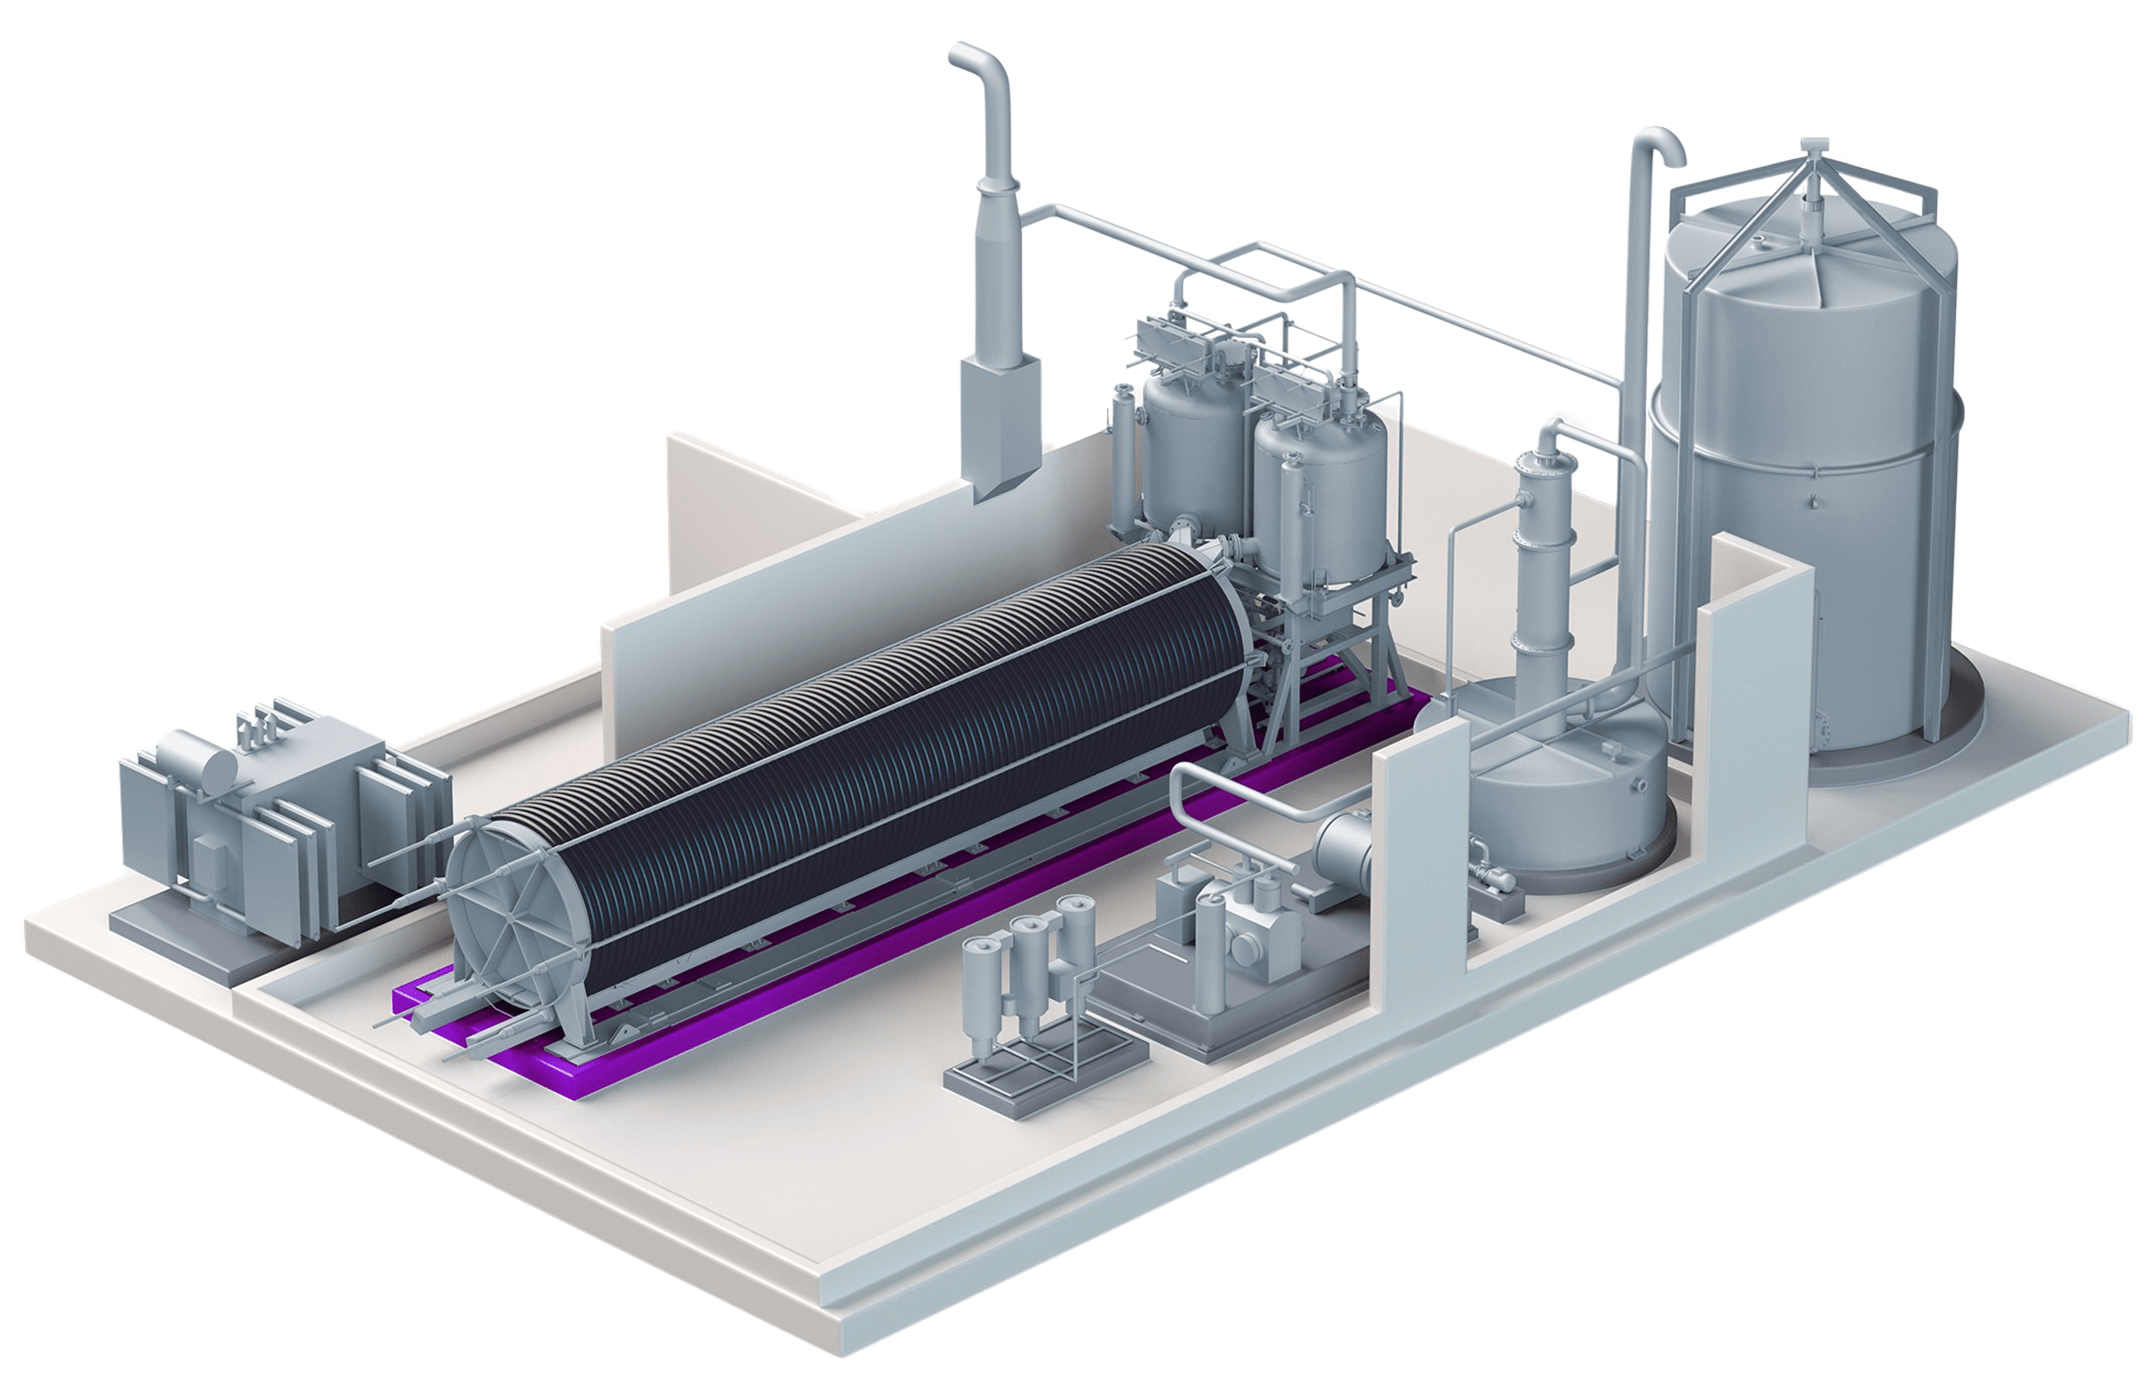
\includegraphics[width=.55\textwidth]{figures/elektrolyzer_nel.png}
    \caption[Alkalický elektrolyzér \enquote{A485} firmy \textit{Nel ASA}]{Alkalický elektrolyzér \enquote{A485} firmy \textit{Nel ASA} \cite{NelASA2018}.} \label{fig:elektrolyzer_nel}
\end{figure}

\subsection{Elektrolýza s protonově vodivou membránou}

\acs{PEM} elektrolýza byla vyvinuta v druhé polovině 20. století, především z důvodu eliminace nevýhod, které má alkalická elektrolýza vody. Reakce na anodě a katodě probíhájí ve vyšší rychlosti než u alkalické elektrolýzy kvůli vysoce aktivnímu povrchu katody (\ce{Pt}) a anody (\ce{IrO2}) a nižší hodnotě pH elektrolytu. Další výhodou \acs{PEM} elektrolýzy je úspora místa. Povrchy obou elektrod mohou být až 10x menší a i tak umožňují vyšší rychlosti probíhajících reakcí, která samozřejmě vede k dosáhnutí vyšší účinnosti celého zařízení. \cite{Tkac2017,Kumar2022} 

PEM elektrolýza vody probíhá při teplotách v rozmezí $30\div80\ \mathrm{^{\circ}C}$ a velikosti provozního napětí $1,4 \div 2,5\ \mathrm{V}$. Proces elektrolýzy začíná na anodové straně, kde dochází k rozkladu vody na kyslík, protony a elektrony. Zatímco je kyslík odváděn, protony procházejí membránou, která umožňuje průchod pouze kladně nabitým iontům, které putují katodovou stranu. Na katodě se protony redukují na vodík. \cite{Kumar2022}
\begin{figure}[ht]
    \centering
    \begin{tikzpicture}
\node[inner sep=0pt] (obrazek) at (0,0)
    {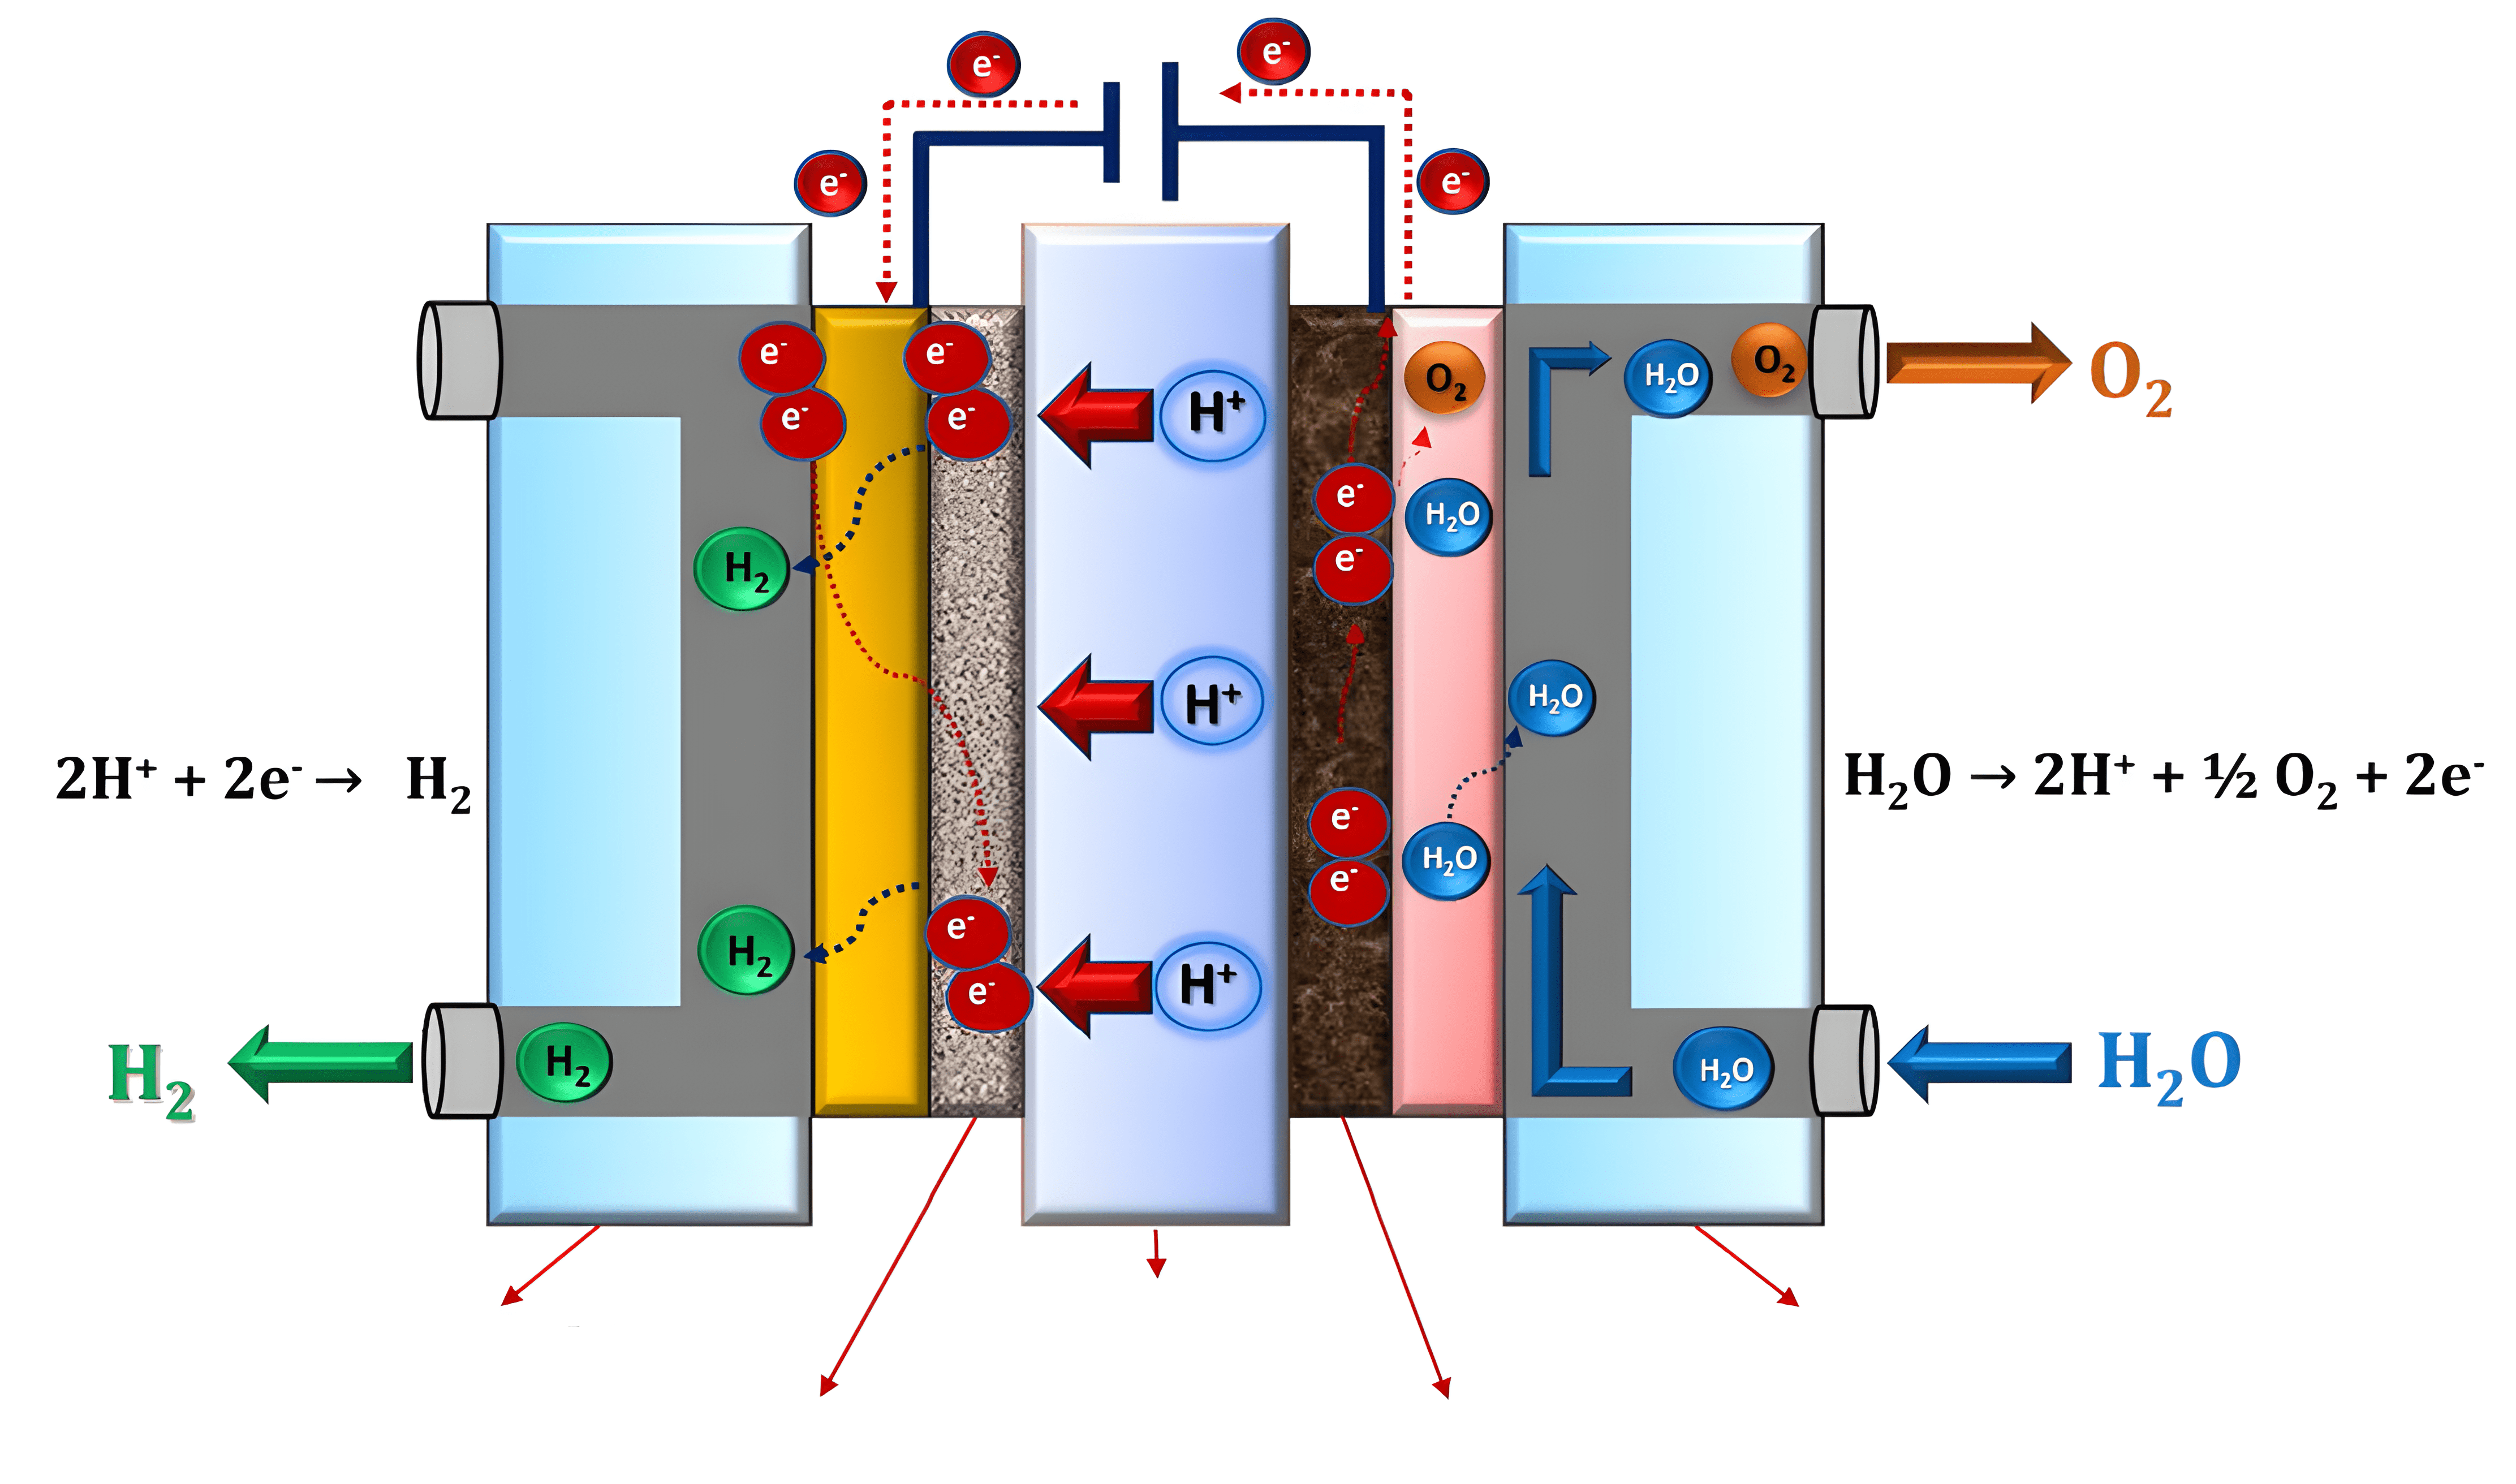
\includegraphics[width=0.9\textwidth]{figures/elekt_pem.png}};
\node[font=\scriptsize] at (3.8,-3.1) {oddělovací desky průtokového pole};
\node[font=\scriptsize] at (-4.7,-3.1) {oddělovací desky průtokového pole};
\node[font=\scriptsize] at (-0.45,-2.9) {membrána};
\node[font=\scriptsize] at (-2.2,-3.5) {katoda};
\node[font=\scriptsize] at (0.9,-3.5) {anoda};
\end{tikzpicture}
    \caption[Schéma principu fungování PEM elektrolýzy vody]{Schéma principu fungování PEM elektrolýzy vody \cite{Kumar2022}.} \label{fig:elekt_pem}
\end{figure}

\noindent
Základní princip \acs{PEM} elektrolyzéru vody je znázorněn na Obr. \ref{fig:elekt_pem} i s vypsanými probíhajícími reakcemi. Spotřeba elektrické energie je u metody \acs{PEM} nižší, ale investiční náklady na pořízení \acs{PEM} elektrolyzéru jsou přibližně $1,5$ krát vyšší než u alkalického elektrolyzéru. To je zapříčiněné vysokými cenami použitých drahých kovů u elektrod a ostatních součástí. \cite{Kumar2022}

K významným globálním výrobcům, kteří se specializují nejen na elektrolyzéry s protonově vodivou membránou, se řadí například německá společnost \textit{Siemens Energy AG}. Jejich elektrolyzér s obchodním názvem \enquote{Silyzer 300} je schopný produkovat $100 \div 2000\ \mathrm{kg}$ vodíku za hodinu při účinnosti celého elektrolyzéru až $75,5\%$. \cite{SiemensEnergy2020}
\begin{figure}[ht]
    \centering
    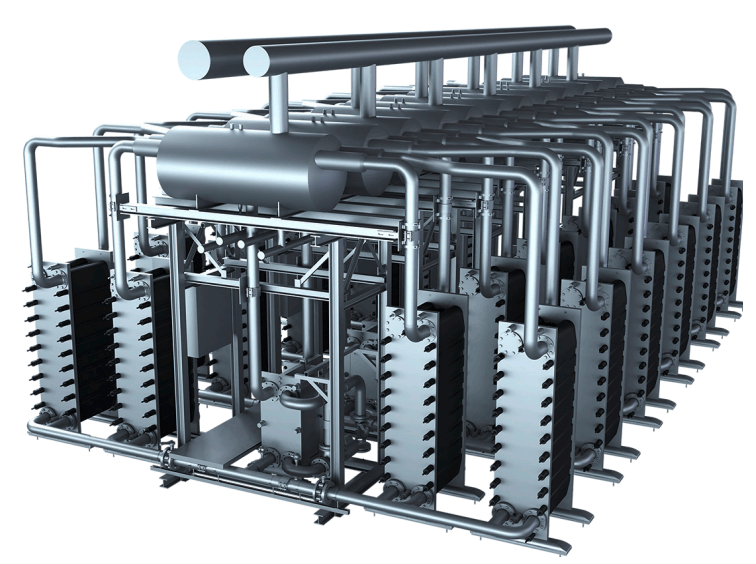
\includegraphics[width=.47\textwidth]{figures/elektrolyzer_siemens.png}
    \caption[PEM elektrolyzér \enquote{Silyzer 300} firmy \textit{Siemens Energy AG}]{PEM elektrolyzér \enquote{Silyzer 300} firmy \textit{Siemens Energy AG} \cite{SiemensEnergy2020}.} \label{fig:elektrolyzer_siemens}
\end{figure}

\subsection{Elektrolýza s pevným oxidem}

Elektrolýza s pevným oxidem, na rozdíl od obou výše zmíněných technologií, probíhá v pásmu vysokých teplot $500\div850\ \mathrm{^{\circ}C}$. Tento fakt přispívá ke zvýšení účinnosti, zlepšení reakční kinetiky a snížení spotřeby elektrické energie na štěpení vody, která je předehřívaná tepelnou energií. Další výhodou této technologie je absence používání elektrod z ušlechtilých drahých kovů. Jako elektrolyt se používá sloučenina oxidu zirkoničitého (\ce{ZrO2}) a oxidu ytritého (\ce{Y2O3}), který má vysoká iontová vodivost, jež implikuje dobrou chemickou a tepelnou stabilitu. \cite{Tkac2017,Kumar2022}
\begin{figure}[h]
    \centering
    \begin{tikzpicture}
\node[inner sep=0pt] (obrazek) at (0,0)
    {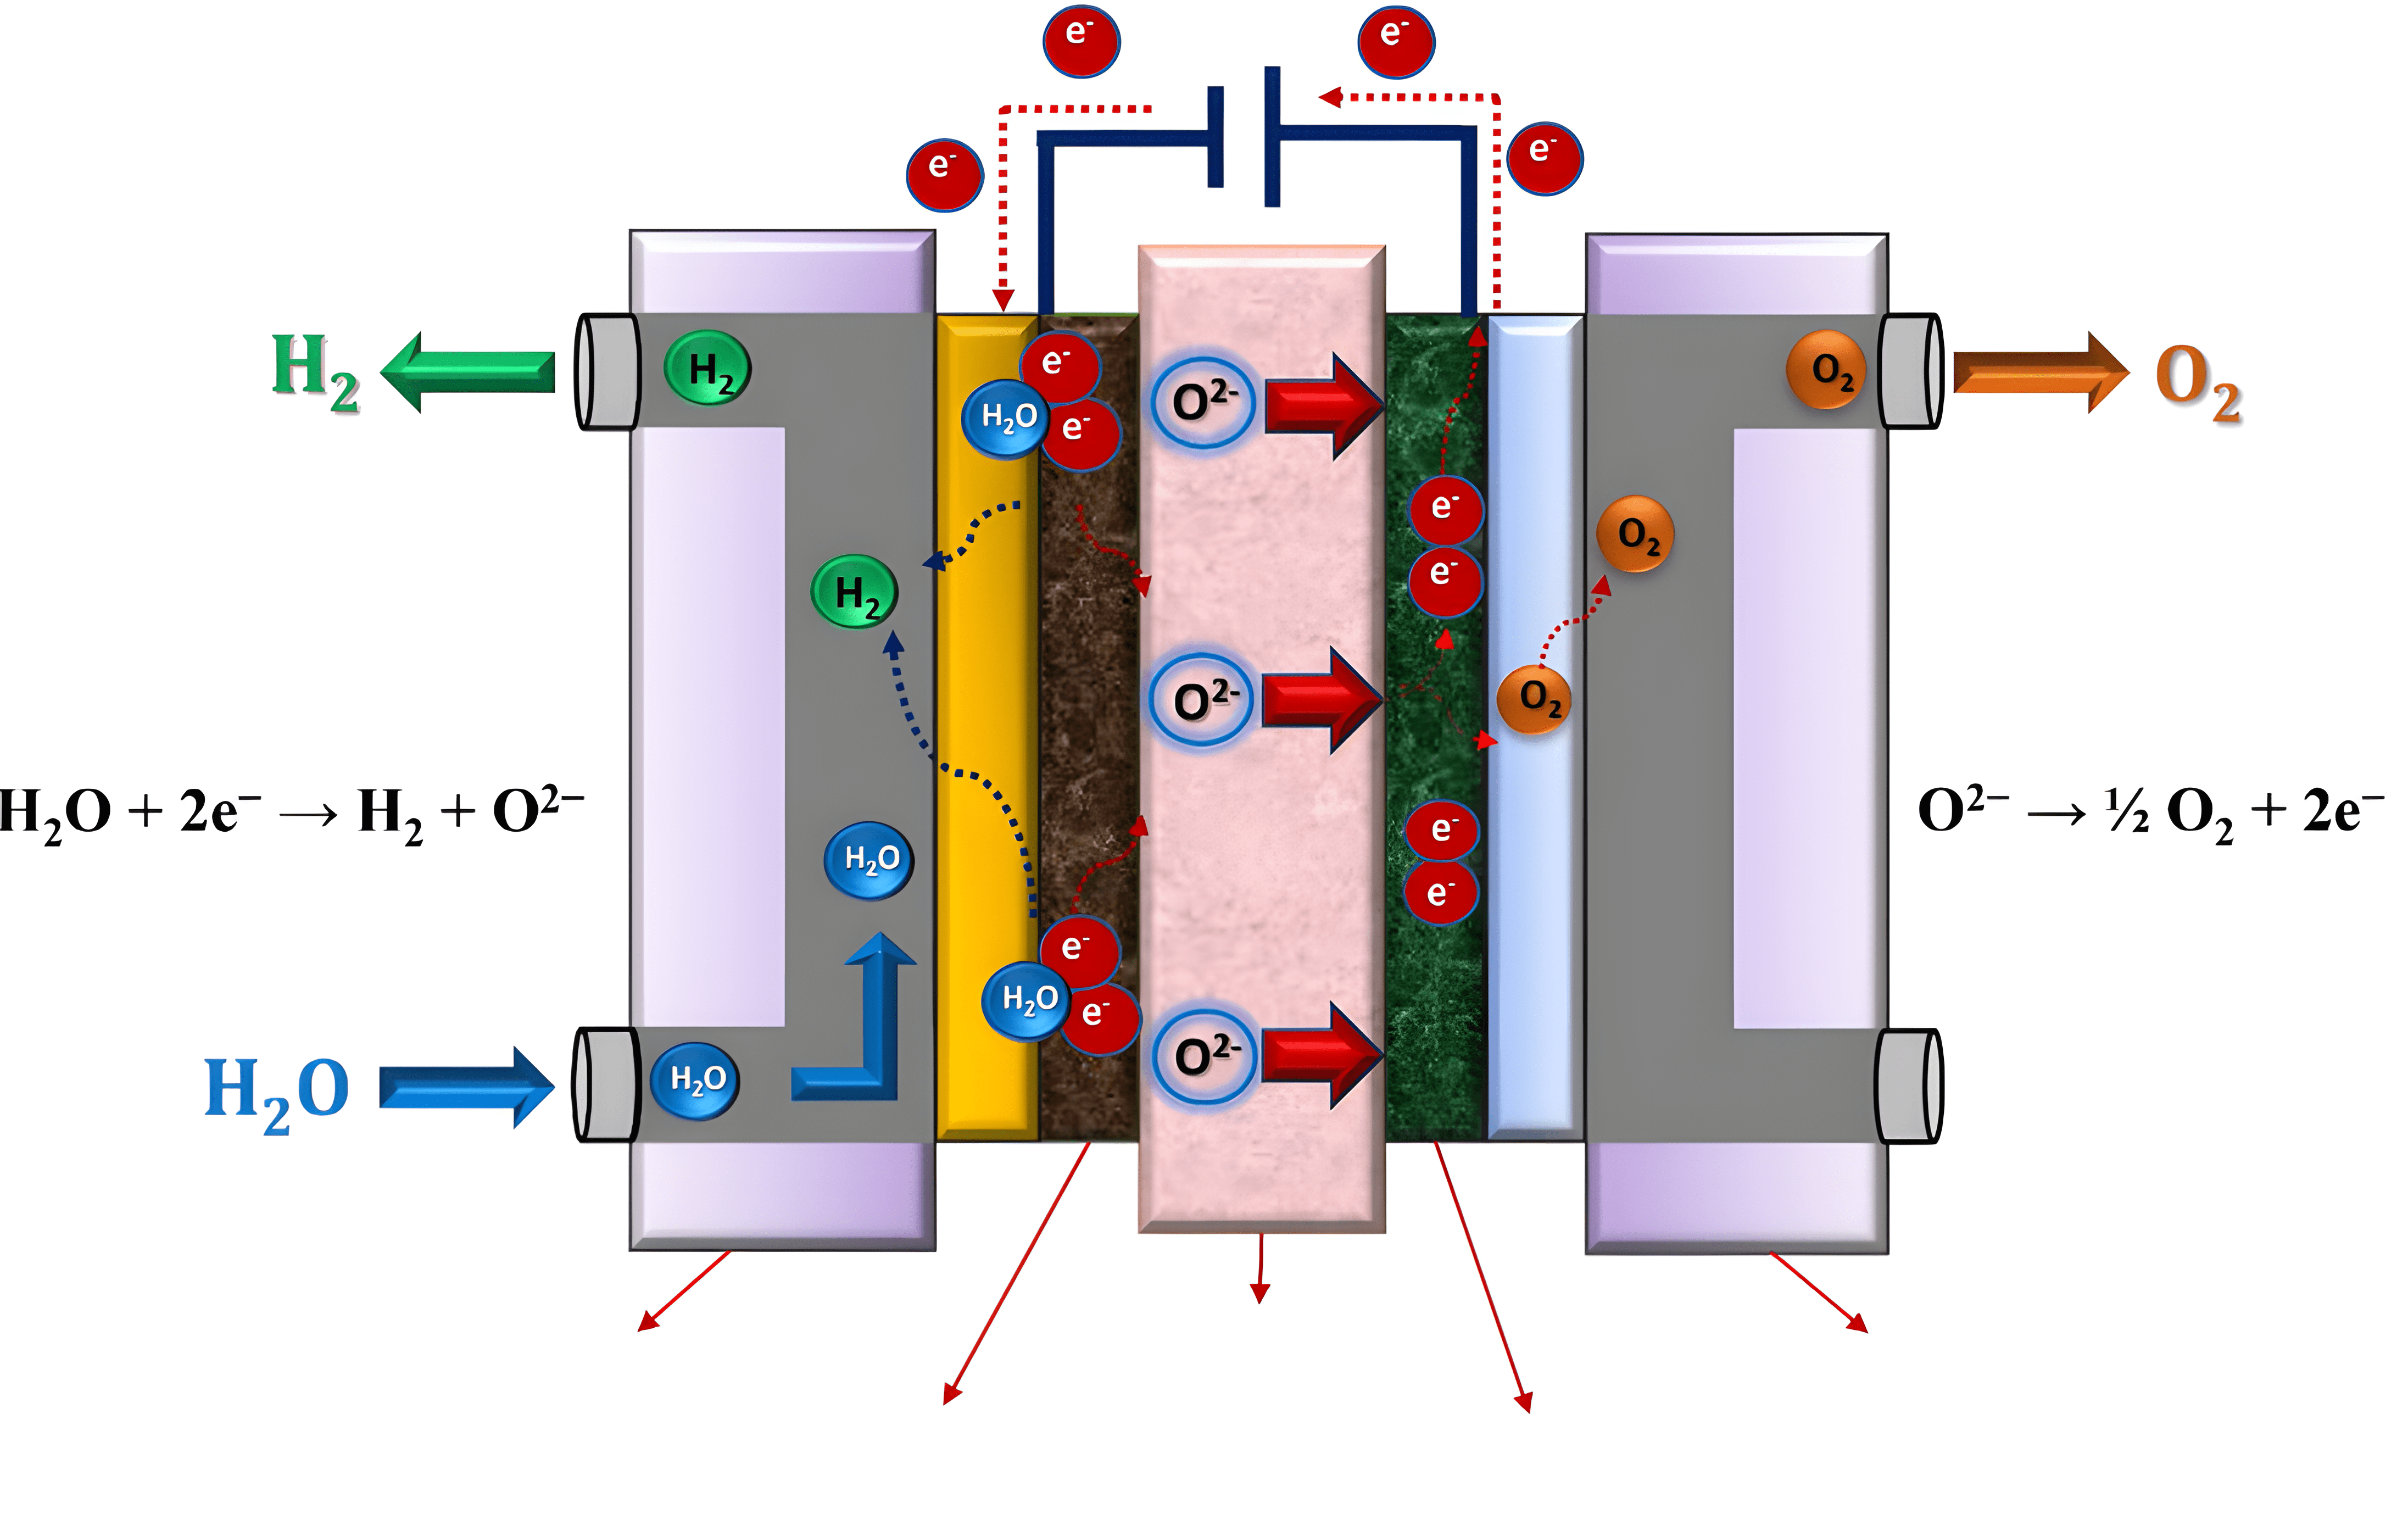
\includegraphics[width=0.85\textwidth]{figures/elekt_soec.png}};
\node[font=\scriptsize] at (4.2,-3.1) {oddělovací desky průtokového pole};
\node[font=\scriptsize] at (-4.1,-3.1) {oddělovací desky průtokového pole};
\node[font=\scriptsize] at (0.2,-2.9) {membrána};
\node[font=\scriptsize] at (-1.2,-3.4) {katoda};
\node[font=\scriptsize] at (1.55,-3.4) {anoda};
\end{tikzpicture}
    \caption[Schéma principu fungování SOEC elektrolýzy vody]{Schéma principu fungování SOEC elektrolýzy vody \cite{Kumar2022}.} \label{fig:elekt_soec}
\end{figure}

\noindent
Proces elektrolýzy začíná na straně porézní katody, kde se molekuly vody redukují na vodík a kyslíkové ionty. Kyslíkové ionty následně putují přes membránu na anodovou stranu, kde za vzniku elektronů oxidují na kyslík. \cite{Kumar2022} Základní princip \acs{SOEC} elektrolyzéru je znázorněn na Obr. \ref{fig:elekt_soec} i s vypsanými probíhajícími reakcemi.

Používání technologie elektrolýzy s pevným oxidem s sebou bohužel přináší i značné nevýhody. Cena používaných keramických materiálů, nízká životnost a doba provozu vede k méně častému využívání. Jedná se však o jednu z nejméně vyvinutých technologií s dobrým potenciálem na budoucí eliminování těchto nevýhod s probíhajícím průzkumem různých výzkumných institucí, které se snaží optimalizovat a vyrovnat náklady na výrobu vodíku. \cite{Kumar2022}

Německá společnost \textit{Sunfire GmbH} patří mezi prominentní světové výrobce elektrolyzérů, včetně těch fungujících na principu pevného oxidu. Jako jedni z mála zaručují dlouhodobý provoz a účinnost až $84\%$. Při jmenovitém výkonu stejnosměrného proudu $2680\ \mathrm{kW}$ a spotřebě $3,6\ \mathrm{kWh}$ elektrické energie na vyrobený $\mathrm{Nm^3}$ vodíku je elektrolyzér \enquote{Sunfire-Hylink SOEC} schopný produkovat až $750\ \mathrm{Nm^3}$ vodíku za hodinu. \cite{SunfireGmbH2021}
\begin{figure}[ht]
    \centering
    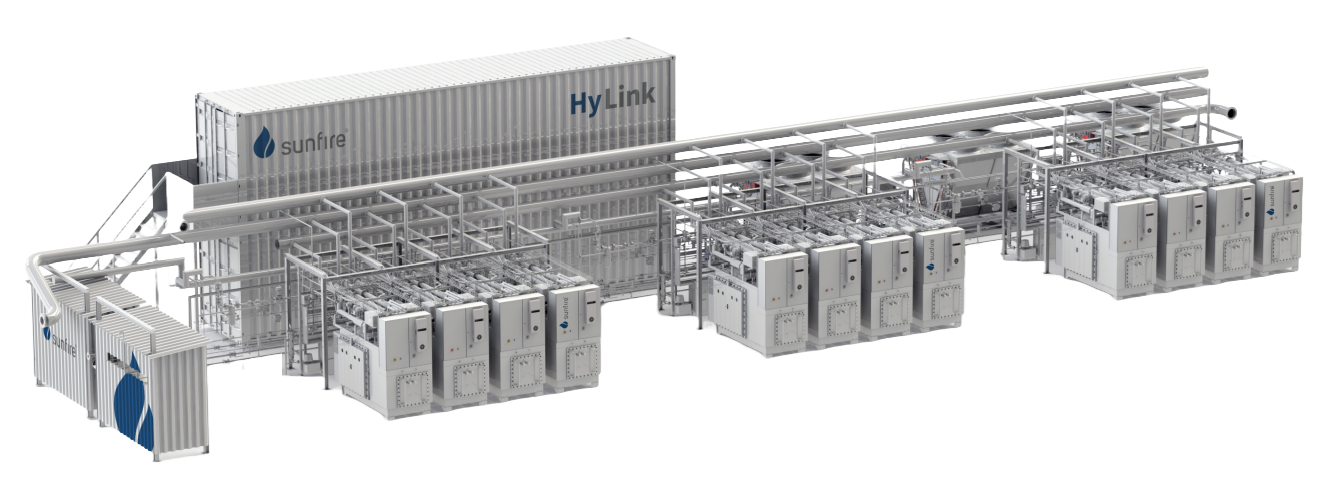
\includegraphics[width=.8\textwidth]{figures/elektrolyzer_sunfire.png}
    \caption[SOEC elektrolyzér \enquote{Sunfire-Hylink SOEC} firmy \textit{Sunfire GmbH}]{SOEC elektrolyzér \enquote{Sunfire-Hylink SOEC} firmy \textit{Sunfire GmbH} \cite{SunfireGmbH2021}.} \label{fig:elektrolyzer_sunfire}
\end{figure}